%!TEX root = ../../thesis.tex

Liquids are made of atoms and molecules. Visualising liquids this way makes understanding a liquid system easier. This thesis is concerned with the behaviour of liquid at the atomic scale.

\section{Liquids at scale}
At the macro scale, the behaviour of liquid is simple and calculable. Modern computers can simulate the movement of liquids using the Navier-Stokes equations with accuracy and speed. This does not hold true when modelling fluid at the scale of individual atoms and molecules, where the behaviour is determined purely by electrical interactions. These interactions are chaotic and therefore simulation of any reasonable sized volume demands prohibitive computing resources.

Water is a liquid comprised of the molecule $H_{2}O$. This molecule is polar, meaning one side has a net positive charge and the other is net negatively charged. This simple fact is responsible for very complex behaviour when dealing with a liquid body of reasonable size.

\begin{figure}
    \begin{center}
        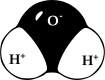
\includegraphics{content/introduction/graphics/polarWater}
    \end{center}
    \caption{A single polar water molecule}
    \label{fig:waterMolecule}
\end{figure}

This thesis, in essence, investigates interactions that take place at the boundary between a liquid and a solid. These interactions take place primarily on the liquid side of the boundary within a volume termed the double layer. The electric field of the solid's interior would be affected by the accumulation of charge at its surface, but this should not affect the analysis of the exterior layer. It is important to note that a solid in the context of this thesis is not simply the walls of a container, but may also refer to solid particles, even molecules, within a liquid. This is the case for emulsified substances such as paints where the formed double layer determines the stability of the emulsion.

This thesis focusses on two applications of interfacial double layers with respect to electrical engineering. Firstly, it looks at a method of harvesting power from water by way of a mechanism that has no moving parts; and secondly, it models the electrical impedance that is seen by a medical implant when placed inside a biological system. The second application is where the majority of the research effort can be found.

\subsection{The Promise of Molecular simulation}
Physical simulations involving the properties of materials and interactions with radio-waves are a common tool for any RF engineer. There are many areas in science and engineering that benefit from powerful computer simulation. Many modern-day computer games simulate the position and velocity of thousands of objects, such as bullets and buildings breaking apart, in near real-time.

These kinds of simulations generally involve calculating the state of a system of objects at a specific time, then adjusting the all of the parameters based the physics of that system at a specific time, and repeating this process for as long as the simulation need continue.

Finite-difference time-domain (FDTD) simulation is a common technique for calculating electrical fields and resulting currents and voltages in the field of electrical engineering. Such simulations can involve hundreds of thousands, \emph{sometimes millions}, of objects. Generally these objects are elements of a 3D mesh that has been created to represent the geometry of the system to be simulated. In such a simulation, each mesh element at every time step needs its various parameters (e.g. temperature, electromagnetic fields, electrical current and voltage) to be calculated based on the parameters of neighbouring objects in the mesh. Because of the dependence on neighbouring parameter values, each time-step may take many passes over each element in a system to calculate the final state before moving on. These sorts of simulations are extremely valuable for the radio frequency engineer as systems of a practical size can be simulated relatively quickly on modest computing hardware.

At this point it seems natural to assume that we could model the behaviour of atoms and molecules in a liquid. Doing this would allow simulation of the interactions that take place at the fluid-soild boundary. It is possible to run such molecular dynamics (MD) simulations, however the number of atoms and molecules in any practical sized volume of fluid is astronomical.

The molar mass of water is defined as $18.0528\thinspace g/Mol$, which represents the amount of water in moles per gram. One gram of water is defined as one millilitre so we can say that for every millilitre of water we have we have an eighteenth of a mole of water. Avagadro's constant, the number of constituent particles per mole of a given substance, is $6.0221\thinspace \times 10^{23}$. Therefore we have one eighteenth of Avagadro's constant in water molecules, which is about $3.3333\times 10^{22}$ molecules. That is 33 333 333 333 333 333 333 333 molecules! The behaviour of double layers in the applications of this research require a far greater volume than $1\thinspace ml$ to be useful, putting molecular simulation out of the picture for the applications discussed in this thesis for the foreseeable future.
